\documentclass[a4paper]{article}
\usepackage[a4paper]{geometry}
\geometry{hscale=0.85,vscale=0.85,centering}
\usepackage[utf8]{inputenc}
\usepackage{amsmath}

\usepackage{graphicx}

\title{Sergej}
\begin{document}
\maketitle

\tableofcontents

\newpage

\section{Qu'est-ce que c'est?}

Sergej est un modèle neuronal numérique que nous appellerons "Cerveau" bien que ce n'en soit pas vraiment un.\\
Il suit des lois de connections qui modifient sa structure interne par le biais de rétroactions.

\section{Sergej et son environnement}

Sergej a besoin de signaux en entrée pour en restituer en sortie.
\begin{figure}
\centering
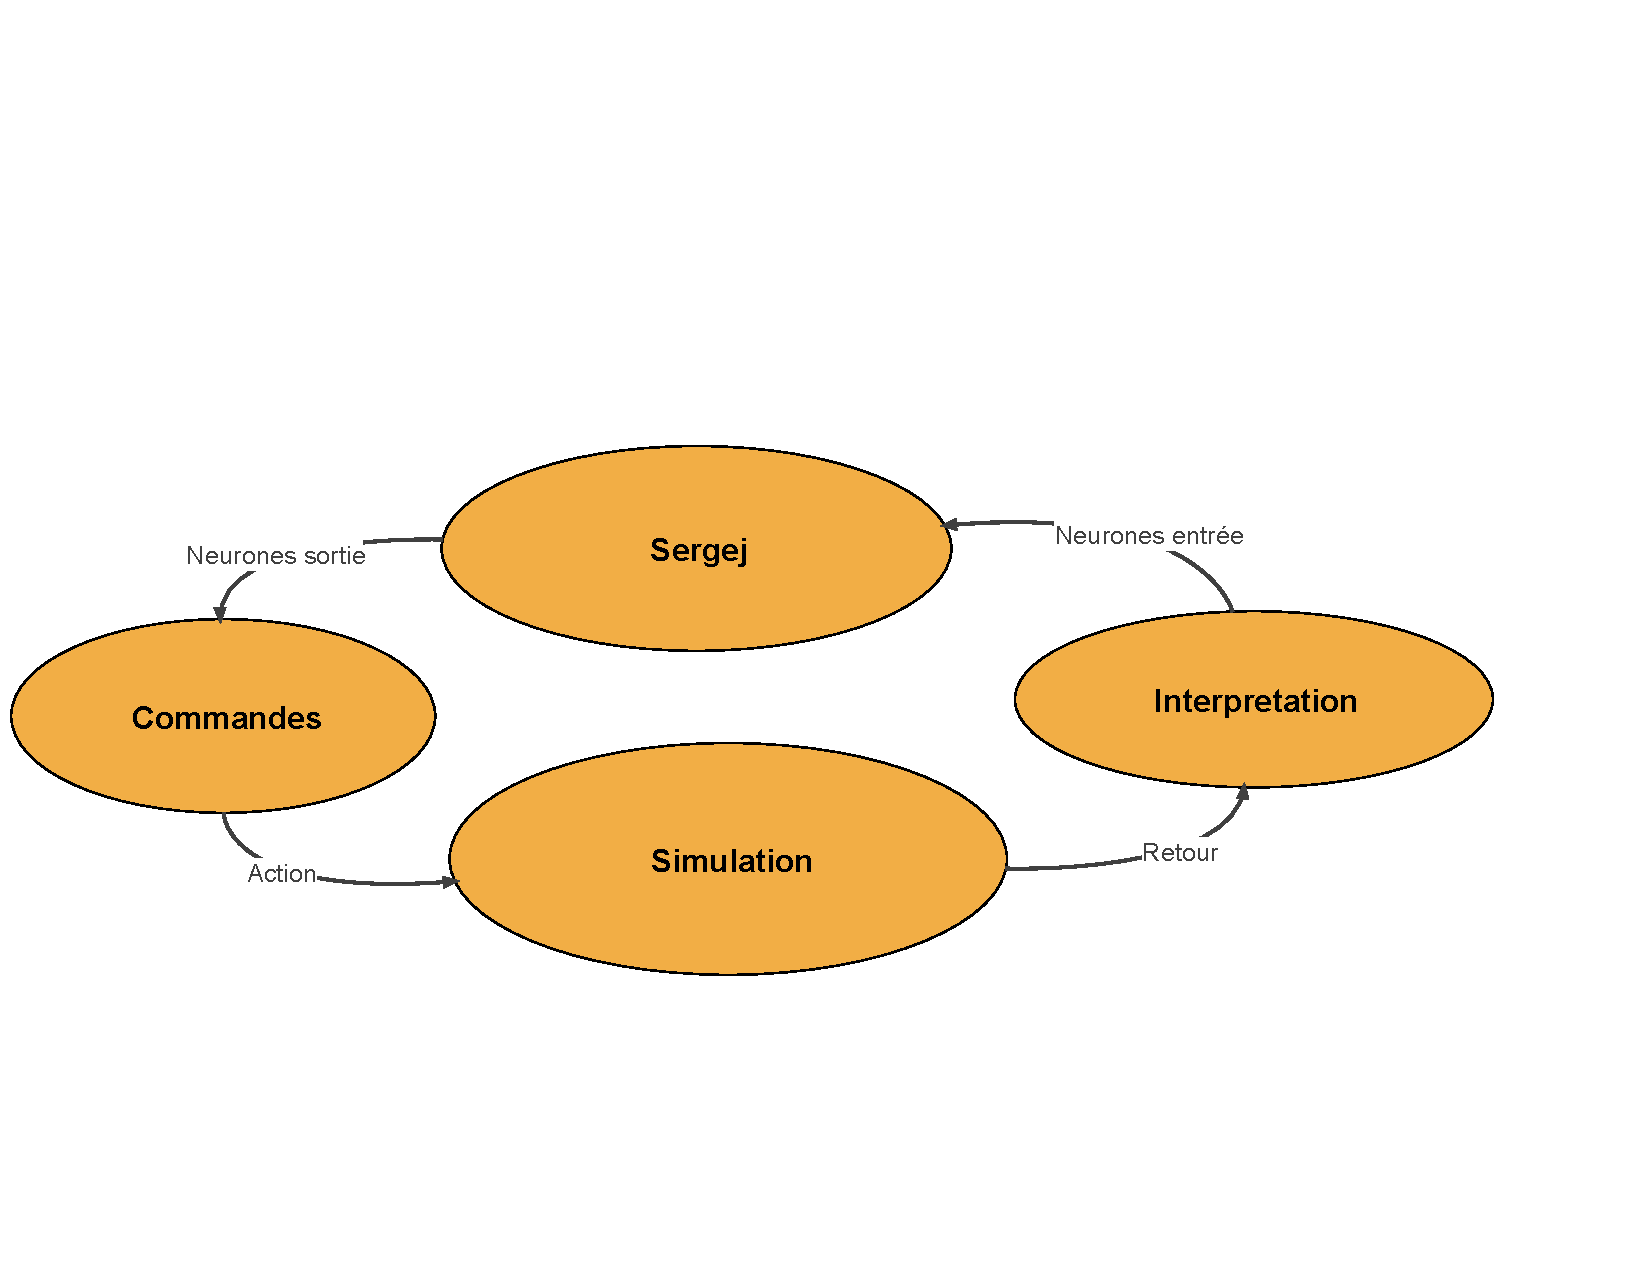
\includegraphics[scale=0.5]{System_commande_diagrame}
\caption{Sergej représenté dans son environnement}
\end{figure}

Le signal en entrée est transmit aux composantes internes de Sergej sommairement appelées neurones. Ces derniers, de même que Sergej reçoivent un signal en entrée pour en fournir un autre en sortie. Néanmoins à ce niveau un même neurone peut transmettre un signal à plusieurs congénères et de même pour ses entrées.

\begin{figure}
\centering
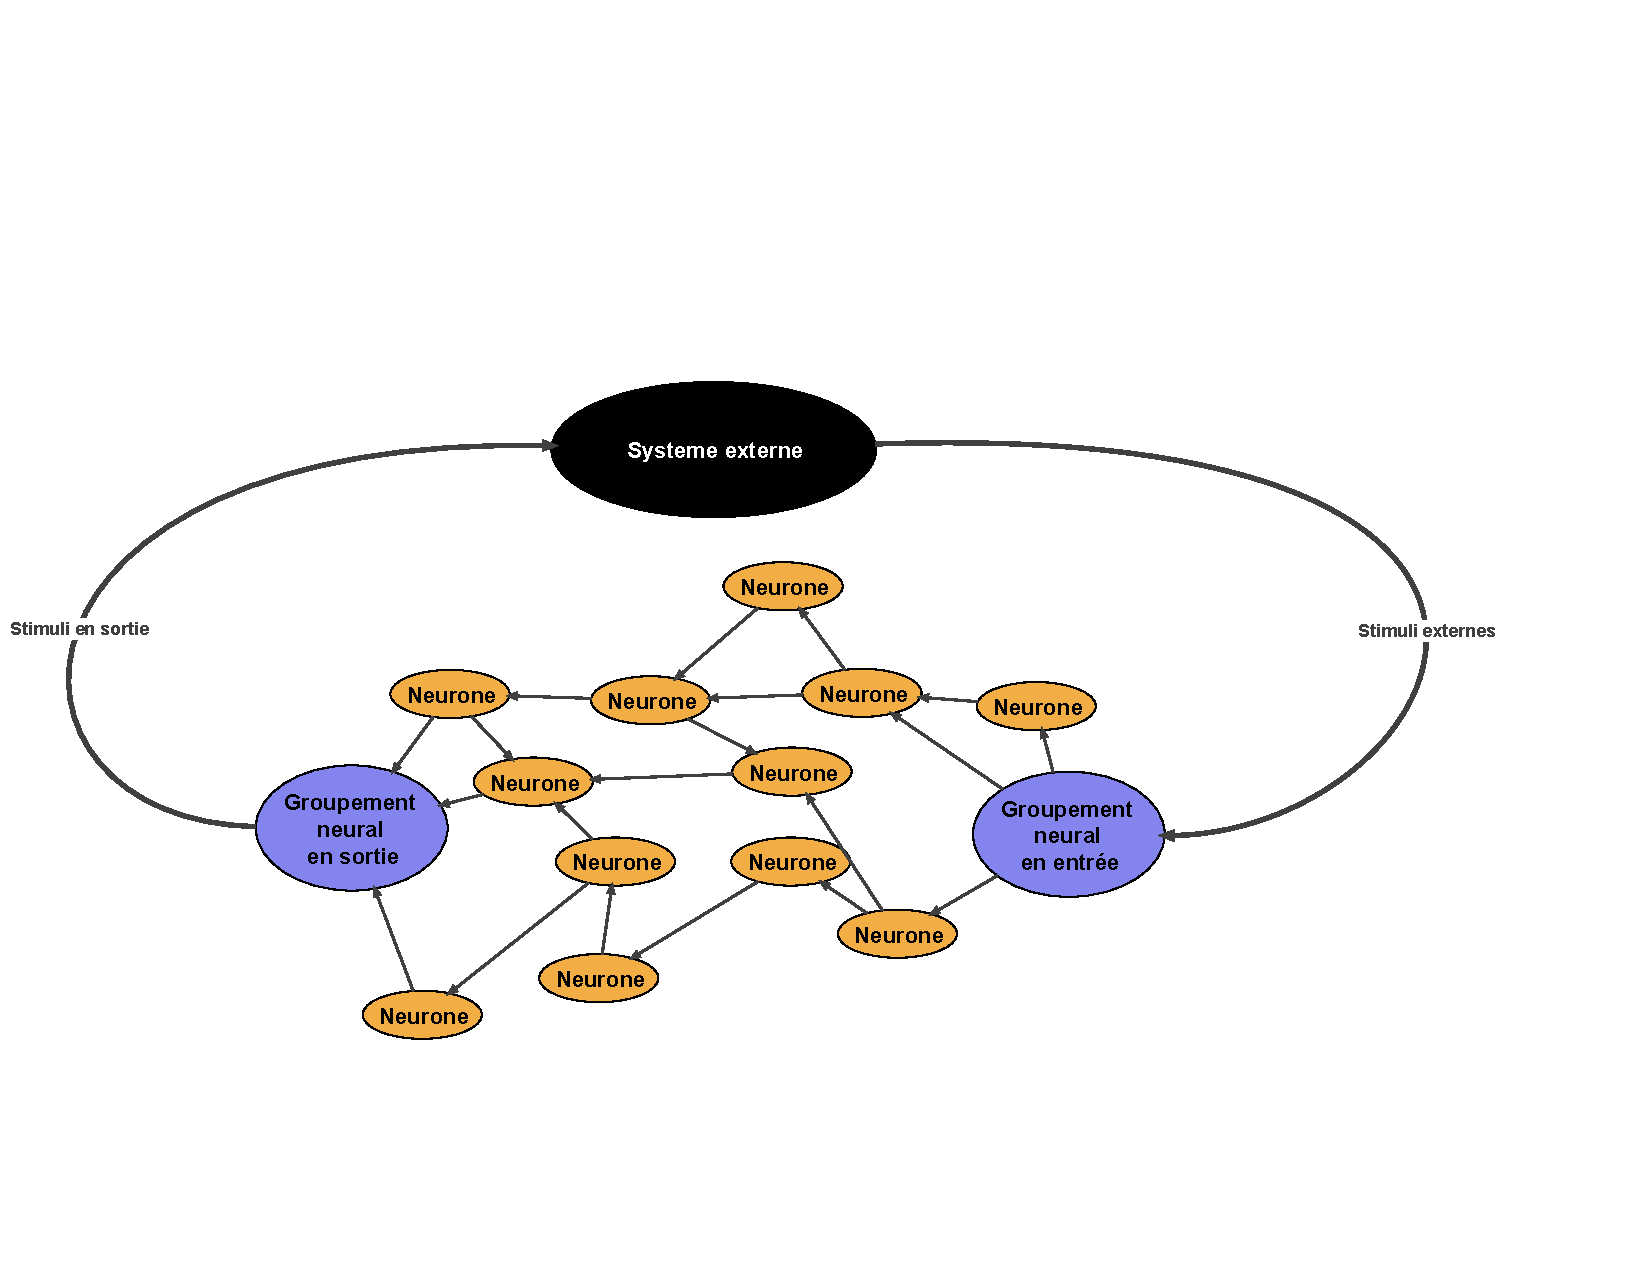
\includegraphics[scale=0.5]{Groupement_neural}
\caption{Schéma de l'architecture neurale interne}
\end{figure}

Sergej ne serait-il pas qu'un seul grand neurone? La question reste en suspend..

\section{Loi de génération et de positionnement}

Les groupements neuraux en entrée et en sortie doivent être générés \textit{avant} les autres afin de permettre à Sergej de communiquer avec son environnement. Par contre les neurones intermédiaires suivent des loi de génération et de positionnement.
\subsection{Loi de génération}
Exemples de lois de génération $G()$:
\begin{itemize}
\item Génération indépendante: Dans ce cas la génération de neurones dépend d'une loi externe au système dépendant, par exemple du temps. \\$G(t)=constante$, le nombre de neurones ajouté est toujours le même.\\
 $G(t)=\alpha\ln (t)$ le nombre de neurones ajoutés croit de moins en moins vite, etc...
\item Génération proportionnelle: Le nombre de neurones ajoutés dépend du nombre de neurones déjà présents.\\ $G(n) = K\left(\dfrac{1-\dfrac{n}{K}}{\alpha}\right)$ avec $\alpha\geq1$. Le nombre de neurones tend vers $K$.\\
\item Génération sur demande: Sergej dispose d'une commande générant des neurones.
\end{itemize}
\subsection{Loi de positionnement}

Une foi généré, un neurone doit être placé dans le réseau.

\end{document}